\begin{frame}{Strategie}
    Testowanie na podstawie właściwości nie jest proste w zastosowaniu, przynajmniej przy pierwszej próbie.
    Istnieją jednak pewne schematy wskazujące drogę, jak stworzyć takie testy.
    \begin{enumerate}[<+->]
        \item Różne ścieżki, ten sam wynik
        \item Tam i z powrotem
        \item Są rzeczy niezmienne
        \item Z czasem rzeczy przestają się zmieniać
        \item Dziel i rządź
        \item Łatwiej zweryfikować niż zaimplementować
        \item Testowanie z wyrocznią
    \end{enumerate}
\end{frame}

\begin{frame}{Strategie - Różne ścieżki, ten sam wynik}
    \begin{columns}[t]
        \column{.5\textwidth}
            Jedną z podstawowych strategii skorzystanie z komutatywności niektórych operacji. Można to zrobić poprzez wykonanie operacji w różnej kolejności.\\
            \onslide<2->{
                Przykładem takiej strategii może być komutatywność dodawania, gdzie wykorzystano \texttt{add x y}, jak i odwrotność tej operacji \texttt{add y x}.\\ 
            }
            \onslide<3->{
                Innym przykładem jest test metody \texttt{sort} danej listy. 
                Wykonanie sortowania, a następnie dodanie do każdego elementu listy \texttt{1} powinno dać taki sam efekt jak dodanie \texttt{1} do każdego z elementów listy, a następnie jej posortowanie.
            }
        \column{.5\textwidth}
        \centering
        \begin{figure}
            \centering
            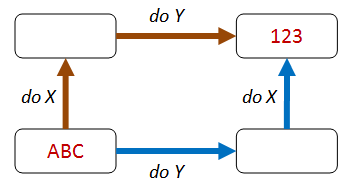
\includegraphics[width=1\textwidth]{images/property_commutative.png}
            \caption{Strategia - komutatywność}
            \label{fig:commutative_strategy}
        \end{figure}    
    \end{columns}
\end{frame}

\begin{frame}{Strategie - Różne ścieżki, ten sam wynik}
    \begin{columns}[t]
        \column{.5\textwidth}
            Jedną z podstawowych strategii skorzystanie z komutatywności niektórych operacji. Można to zrobić poprzez wykonanie operacji w różnej kolejności.\\
            Przykładem takiej strategii może być komutatywność dodawania, gdzie wykorzystano \texttt{add x y}, jak i odwrotność tej operacji \texttt{add y x}.\\ 
            Innym przykładem jest test metody \texttt{sort} danej listy. 
            Wykonanie sortowania, a następnie dodanie do każdego elementu listy \texttt{1} powinno dać taki sam efekt jak dodanie \texttt{1} do każdego z elementów listy, a następnie jej posortowanie.
        \column{.5\textwidth}
        \centering
        \begin{figure}
            \centering
            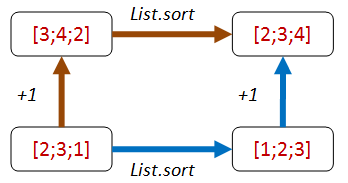
\includegraphics[width=1\textwidth]{images/property_list_sort1.png}
            \caption{Strategia - komutatywność}
            \label{fig:commutative_strategy_example}
        \end{figure}    
    \end{columns}
\end{frame}

\begin{frame}{Strategie - Tam i z powrotem}
    \begin{columns}[t]
        \column{.5\textwidth}
            Przykładem takiego testu mogą być przeciwne operacje matematyczne jak:
            \begin{itemize}[<+->]
                \item \texttt{dodawanie/odejmowanie}
                \item \texttt{mnożenie/dzielenie}
                \item \texttt{potęga/logarytm}.
            \end{itemize} 
            \onslide<4->{Innymi przykładami są operacje niekoniecznie matematyczne:}
            \begin{itemize}[<+->]
                \item \texttt{serializacja/deserializacja}
                \item \texttt{zapis/odczyt z pliku}
                \item \texttt{wstaw/sprawdź czy zawiera}.
                \item \texttt{odwrócenie listy/odwrócenie listy}
            \end{itemize} 
        \column{.5\textwidth}
        \centering
        \begin{figure}
            \centering
            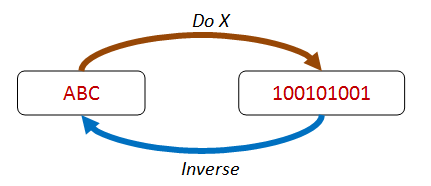
\includegraphics[width=1\textwidth]{images/property_inverse.png}
            \caption{Strategia - inwersja}
            \label{fig:inverse_strategy}
        \end{figure}    
    \end{columns}
\end{frame}

\begin{frame}{Strategie - Są rzeczy niezmienne}
    \begin{columns}[t]
        \column{.5\textwidth}
            Czasami testowana funkcja przetwarzając dane zachowuje część ich właściwości.
            Chociażby funkcje \texttt{sort} lub \texttt{map} wykonane na liście \texttt{n} elementów, zwracaja odpowiednio zmodyfikowaną listę \texttt{n} elementową.
        \column{.5\textwidth}
        \centering
        \begin{figure}
            \centering
            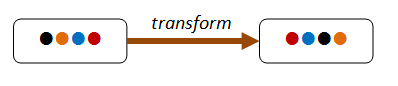
\includegraphics[width=1\textwidth]{images/property_invariant.png}
            \caption{Strategia - niezmienność}
            \label{fig:invariant_strategy}
        \end{figure}    
    \end{columns}
\end{frame}


\begin{frame}{Strategie - Z czasem rzeczy\\przestają się zmieniać}
    \begin{columns}[t]
        \column{.5\textwidth}
            Inną właściwością funkcji może być niezmienność wyniku funkcji po ponownym jej zaaplikowaniu. 
            Innymi słowy, wykonanie funkcji 2 razy daje taki sam efekt, jak jednokrotne jej zaaplikowanie.
            \onslide<2->{Przykładami takich operacji, dla których taki typ testu miałby zastosowanie to metoda \texttt{distinct} wykonana na danej liście, lub wykonanie \texttt{update} na danej bazie danych.}
        \column{.5\textwidth}
        \centering
        \begin{figure}
            \centering
            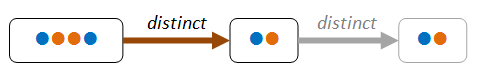
\includegraphics[width=1\textwidth]{images/property_idempotence.png}
            \caption{Strategia - idempotentność}
            \label{fig:independance_strategy}
        \end{figure}    
    \end{columns}
\end{frame}


\begin{frame}[fragile]{Strategie - Dziel i rządź}
    \begin{columns}[t]
        \column{.5\textwidth}
            Istnieją sposoby na testowanie na podstawie właściwości jest wykorzystanie rekursywności struktur przekazywanych do funkcji, takich jak \texttt{listy}, \texttt{drzewa}. 
            \onslide<2->{
                Przykładem może być sprawdzenie za pomocą tej metody funkcji sort.
            }
        \column{.5\textwidth}
            \centering
            \begin{figure}
                \centering
                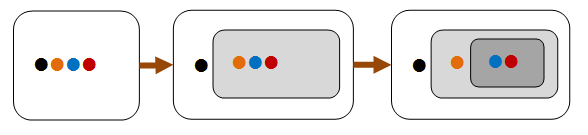
\includegraphics[width=1\textwidth]{images/property_induction.png}
                \caption{Strategia - rekursywna}
                \label{fig:recursive_strategy}
            \end{figure}    
    \end{columns}
\end{frame}

\begin{frame}[fragile]{Strategie - Dziel i rządź}
    \begin{lstlisting}[language=FSharp, xleftmargin=-10pt,xrightmargin=-10pt,numbers=none, basicstyle=\ttfamily\small]
    let rec firstLessThanSecond_andTailIsSorted sortFn 
    (aList:int list) =
    let sortedList = aList |> sortFn
    match sortedList with
    | [] -> true
    | [first] -> true
    | [first;second] -> first <= second
    | first::second::rest->
        first <= second &&
        let tail = second::rest
        // check that tail is sorted
        firstLessThanSecond_andTailIsSorted sortFn tail
    \end{lstlisting}
\end{frame}

\begin{frame}{Strategie - Łatwiej zweryfikować niż\\zaimplementować}
    \begin{columns}[t]
        \column{.5\textwidth}
            Niekiedy testowana funkcja jest skomplikowana, ale jej rezultat da się łatwo sprawdzić. Przykładem może być funkcja wyszukująca wyjście z labiryntu, gdzie sam algorytm wyszukiwania odpowiedniej ścieżki jest skomplikowany, 
            natomiast samo sprawdzenie, czy ścieżka dobrze prowadzi do wyjścia można w łatwy sposób zweryfikować.
        \column{.5\textwidth}
        \centering
        \begin{figure}
            \centering
            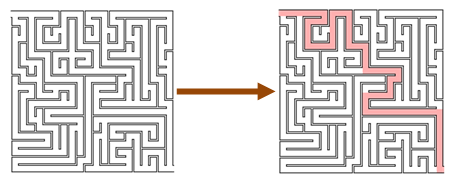
\includegraphics[width=1\textwidth]{images/property_easy_verification.png}
            \caption{Strategia - łatwe sprawdzenie}
            \label{fig:easy_verification_strategy}
        \end{figure}    
    \end{columns}
\end{frame}


\begin{frame}{Strategie - Testowanie z wyrocznią}
    \begin{columns}[t]
        \column{.65\textwidth}
            Zdaża się, że funkcjonalność została już napisana i trzeba ją zrefactorować, przepisać, napisać od nowa. Warto wtedy wykorzystać wartości zwracane przez oryginalnie zaimplementowany algorytm jako pewną wartość wyniku, pewnego rodzaju wyrocznię, uznając go jako prawdę.
            \onslide<2->{W taki sposób można sprawdzić, czy nowa funkcja w pewnym stopniu pokrywa się ze starą funkcją. Czasami też istnieje wiele algorytmów doprowadzających do tego samego wyniku, mające różne złożoności, czy też działające równolegle.}
            \onslide<3->{Można wykożystać wtedy najprostrzy algorytm jako wyrocznię, ze względu na najmniejsze prawdopodobieństwo napisania takiego algorytmu z błędem. Następnie, przy wykorzystaniu wyroczni, stworzyć bardziej skomplikowany (często efektywniejszy) algorytm.}
        \column{.35\textwidth}
        \centering
        \onslide<1->{
        \begin{figure}
            \centering
            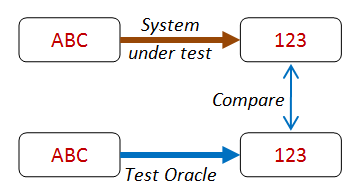
\includegraphics[width=1\textwidth]{images/property_test_oracle.png}
            \caption{Strategia - wyrocznia}
            \label{fig:oracle_strategy}
        \end{figure} 
        }   
    \end{columns}
\end{frame}